%\usepackage{comment}

{\bf [60 points] Motif Finding}\\

In lecture we were introduced to an algorithm used for finding motifs in DNA sequences based on Expectation Maximization (EM). This algorithm forms the basis of the MEME Suite (\textbf{M}ultiple \textbf{E}M for \textbf{M}otif \textbf{E}lucidation), one of the most widely used softwares in genomics. Several good papers are available for understanding the algorithm, including the ones \href{https://www.cs.cmu.edu/~epxing/Class/10810-06/readings/MEME.pdf}{here} and \href{https://tlbailey.bitbucket.io/papers/meme.ml.pdf}{here}.

\\

Consider a biological motif of length $W$, $M = (M_1, \dots, M_W)$, where $M_i \in \{A, C, G, T\}$. Our model for biological motifs is that each $M_i$ is a Multinoulli-distributed random with its own probability distribution over the nucleotides $A, C, G,$ and $T$.
We can equivalently represent this motif as a position weight matrix $(M)_{ij}$, for which 
$$M_{ij} = \mathbb P(M_j = i),$$
where $j = 1, \dots, W$ and $i \in \{A, C, G, T\}$. Consider the PWM below for a motif of length $W=6$: 

\begin{equation}
M = \begin{blockarray}{ccccccc}
& M_1 & M_2 & M_3 & M_4 & M_5 & M_6 \\
\begin{block}{c[cccccc]}
  A & 0.8 & 0.1 & 0 & 0.9 & 0 & 0.3  \\
  C & 0 & 0.4 & 0.05 & 0.03 & 0.1 & 0.2 \\
  G & 0.2 & 0 & 0.95 & 0.02 & 0.1 & 0.1 \\
  T & 0 & 0.5 & 0 & 0.05 & 0.8 & 0.4  \\
\end{block}
\end{blockarray}
\label{q2-motif-pwm}
\end{equation}

One of the key assumptions we make when modeling motifs is that $M_i \perp M_j$ for $i \ne j$; that is, the distributions of the nucleotides in each position of the motif are independent of one another. 

\begin{enumerate}

\item Find the probability $\mathbb P(M = ACCTTA)$.

%%%%%%%%%%%%%%%%%%
\begin{solution}

\end{solution}
%%%%%%%%%%%%%%%%%%

\item  Provide the Consensus Sequence corresponding to the PWM above; i.e., the sequence $m = (m_1, \dots, m_5)$ such that $\mathbb P(M = m)$ is maximized.

%%%%%%%%%%%%%%%%%%
\begin{solution}

\end{solution}
%%%%%%%%%%%%%%%%%%

\item
Which of the following sequence logos accurately represents the PWM? Briefly describe why the other logos are incorrect.

1) 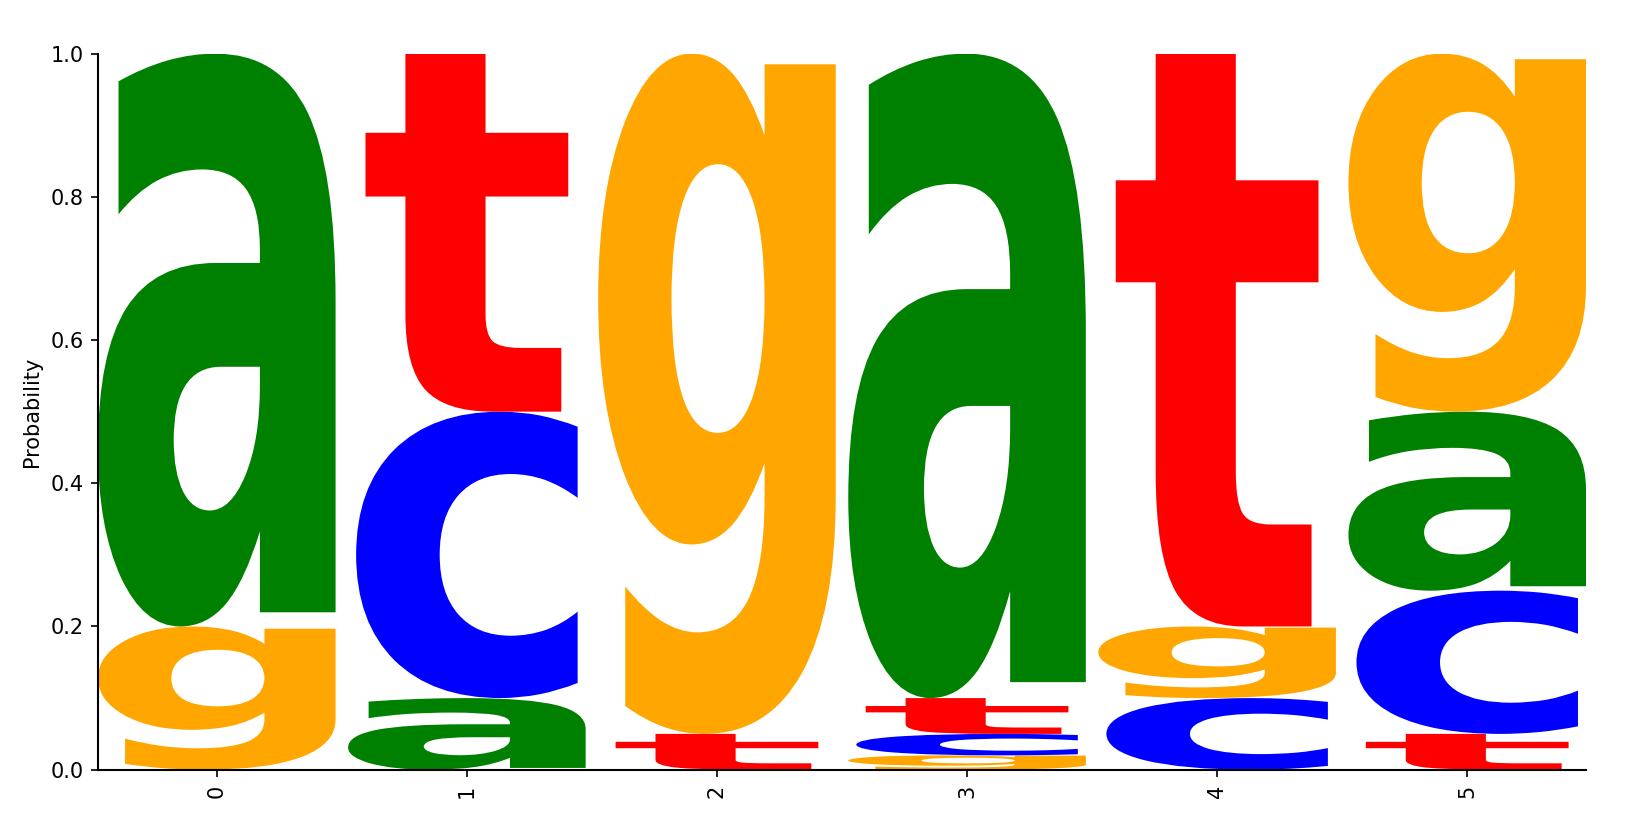
\includegraphics[scale=.2]{figures/logo_1.png} \\
2) 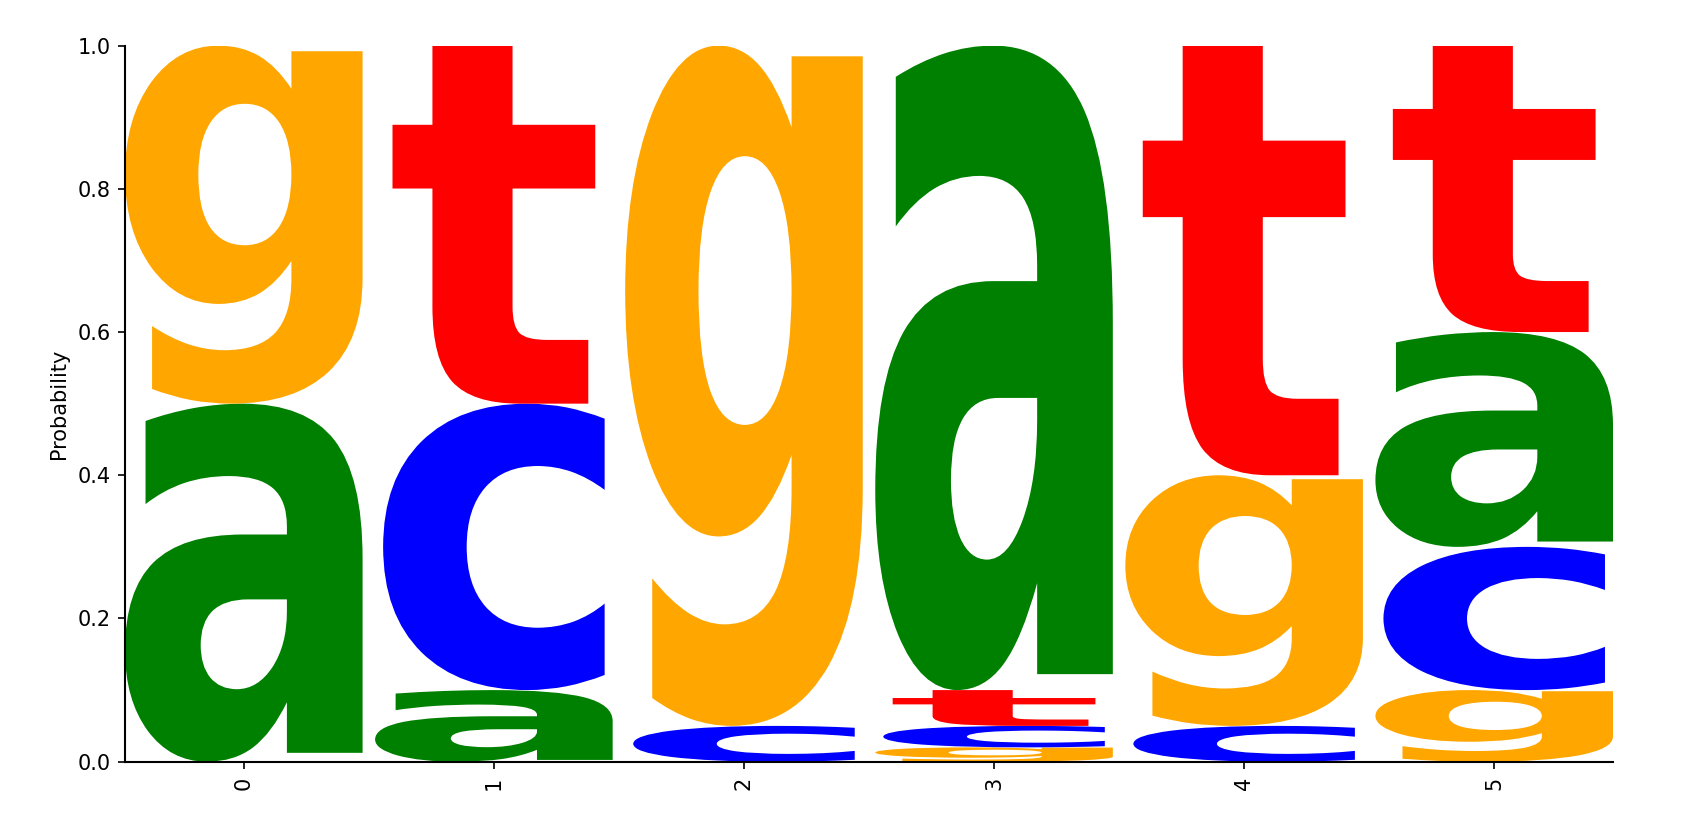
\includegraphics[scale=.2]{figures/logo_2.png} \\
3) 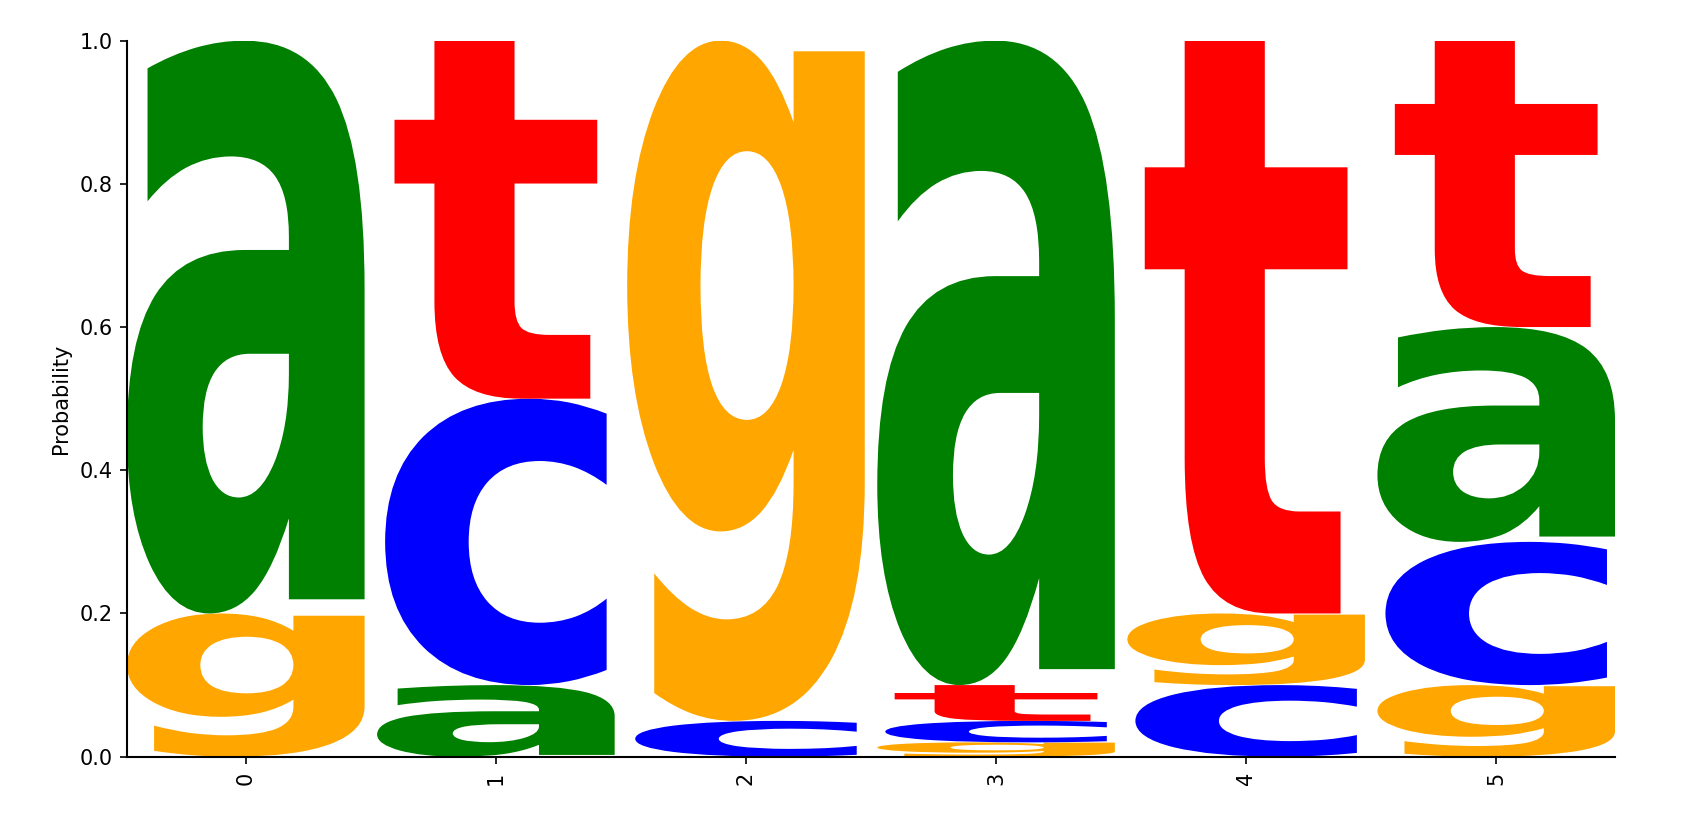
\includegraphics[scale=.2]{figures/logo_3.png}

%%%%%%%%%%%%%%%%%%
\begin{solution}
\end{solution}
%%%%%%%%%%%%%%%%%%

\item 
The height of the sequence logo is often scaled by the information content at a given position i. The information content is given by $R_i = log_2(4) - (H_i + e_n)$, where $H_i$ is the entropy of the position, and $H_i = -\Sigma_j [M_{i,j} * log_2 M_{i,j}]$. \\
Which position in the PWM has the greatest entropy? How is entropy related to conservation?
%%%%%%%%%%%%%%%%%%
\begin{solution}

\end{solution}
%%%%%%%%%%%%%%%%%%

\item One of the advantages of the MEME suite is that, for a given DNA sequence, it can detect the most likely positions to find the motif learned in the PWM. To do so, it converts the PWM into a matrix of log likehood ratios using the formula $LLR(s) = log_2[\frac{Pr(s|M)}{Pr(s|M_{bg}})]$. The log likehood score that a given position i is a start position of the motif is equivalent to $S(X) = \sum_{i=x_i}^{i=x_i+w} log_2[\frac{M_{ij}}{M_{ij}^{bg}}]$. \\

One method of determining if a position is included in the motif is to use a decision rule. For example, we could use : '$X$ is a true instance of $M$ if $LLR(X)$ > 0, or equivalently, if $\mathcal S(X) > 0$'.
Is this a statistically sound approach? Why or why not?

%%%%%%%%%%%%%%%%%%%%%%%
\begin{solution}

\end{solution}
%%%%%%%%%%%%%%%%%%%%%%%

\item An alternative approach to determine where or not a position i contains the motif is to use hypothesis testing to calculate the p-value for S(p). We can define the hypotheses as:
\begin{itemize}
    \item $H_0$: $X$ is drawn from the background distribution $M^{bg}$
    \item $H_1$: $X$ is drawn from the motif distribution $M$ 
\end{itemize}
Briefly describe a method for calculating the test statistic. Hint: one definition of p-value is the probability of receiving a value as or even more extreme than S(X) under the null hypothesis. 

%%%%%%%%%%%%%%%%%%%%%%%%%%%%%%
\begin{solution}

\end{solution}
%%%%%%%%%%%%%%%%%%%%%%%%%%%%%%

\end{enumerate}

